\section{Cinematica Manipolatore}
L'obiettivo di questa sezione è quello di andare ad illustrare le metodologie che ci hanno consentito di ottenere sia la cinematica diretta che quella inversa, entrambe per posizione, velocità ed accelerazione.
\\Prima di proseguire nei paragrafi seguenti andiamo a definire una tabella con i principali parametri del robot:
\begin{table}[h!]
\centering
\begin{tabular}{|c |c |c|} 
 \hline
 Nome & Descrizione  & Valore \\ [0.5ex] 
 \hline\hline
 $l [m]$ & lunghezza link  & 0.25 \\ 
 $m [kg]$ & massa link & 2.9 \\
 $c_m [m]$ & posizione centro di massa & 1.25 \\
 $J_r [kg\cdot m^2]$ & momento d'inerzia baricentrico & $5.22\cdot 10^{-2}$ \\
 $d [m]$ & lunghezza semitelaio & 0.09 \\
 \hline
\end{tabular}
\caption{Parametri manipolatore}
\label{table:1}
\end{table}
Tutti e quattro i link hanno lunghezza, massa, posizione del centro di massa e momento di inerzia uguali, per questo si è deciso di rappresentare i dati una sola volta.
\begin{figure}[ht]
\begin{center}
    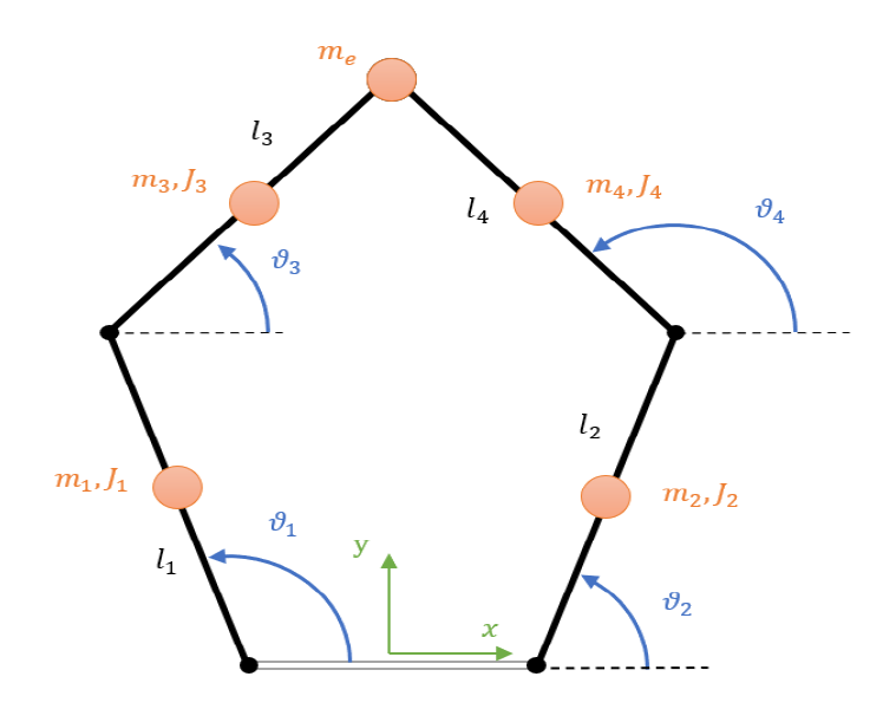
\includegraphics[scale=0.6]{Immagini/Robot2.png}
    \caption{Rappresentazione fisica del robot \label{fig:Robot1}}
\end{center}
\end{figure}
\subsection{Cinematica Diretta}
La cinematica diretta si occupa di trovare il legame tra i parametri interni del robot e la posa che esso assume, per posa si intende la posizione e l'orientamento. In questa sezione andremo ad analizzare la cinematica diretta di posizione, velocità ed accelerazione.
\subsubsection{Posizione}\label{sec:Cinematica-pos}
Nella cinematica diretta di posizione, a partire dal robot e da $\theta_1$ e $\theta_2$, riusciamo a ricavare la posizione dei link non motorizzati, i loro angoli, che sono rispettivamente $\theta_3$ e $\theta_4$ e la posizione $[x,y]$ dell'\textit{end-effector}.
\\L'approccio utilizzato per il calcolo della cinematica diretta è stato quello delle equazioni alle circonferenze, in particolare vengono definite due equazioni
\begin{itemize}
	\item Circonferenza centrata in E1 che passa per l'end-effector e la base del primo link
	\item Ciconferenza centrata in E2 che passa per l'end-effector e la base del secondo link
\end{itemize}
\begin{figure}[ht]
	\begin{center}
		\includegraphics[scale=0.65]{Immagini/EqCirc}
		\caption{Equazioni alle circonferenze \label{fig:eqCirc}}
	\end{center}
\end{figure}
Dalla combinazione di queste due equazioni otteniamo il seguente sistema:
\begin{equation}
    \begin{cases}
    (x-\frac{l}{2}-l\cos\theta_1)^2+(y-l\sin\theta_1)^2 = l^2 \\
    (x+\frac{l}{2}-l\cos\theta_2)^2+(y-l\sin\theta_2)^2 = l^2
    \end{cases}
\end{equation}
Da queste, andando a sviluppare i calcoli possiamo definire i parametri:
\begin{equation*}
    A = l^2 (\sin\theta_2- \sin\theta_1)^2 + (-2 d-l (\cos\theta_2 - \cos\theta_1))^2
\end{equation*}
\begin{equation*}
\begin{aligned}
   B =  -2 l^2 d (\sin\theta_2-\sin\theta_1)  (\cos(\theta_2+\theta_1) + l(\sin\theta_2-\sin\theta_1)   (-2d-l(\cos\theta_2-\cos\theta_1))\\ (-2d-2l\cos\theta_2) - 2l\sin\theta_2 (-2d-l(\cos\theta_2-\cos\theta_1))^2
\end{aligned}
\end{equation*}
\begin{equation*}
\begin{aligned}
    C = l^2 d^2 (\cos\theta_2+\cos\theta_1)^2-l d (\cos\theta_2+\cos\theta_1)(-2d-l(\cos\theta_2-\cos\theta_1) ) \\ (-2d-2l\cos\theta_2)+(d^2+2dl\cos\theta_2)(-2dl(\cos\theta_2-\cos\theta_1))^2
\end{aligned}
\end{equation*}
Il passo successivo è quello di ricavare la posizione $P=[x,y]$ dell'end-effector; si può procedere grazie alla formula risolutiva delle equazioni di secondo grado \begin{equation*}
	s_{1,2}\footnote{$\Delta = \sqrt{b^2-4ac}$} = \frac{-b \pm \Delta}{2a}
\end{equation*}
 Si può notare facilmente che la formula fornisce due risultati diversi, in una caso quando si utilizza $+\Delta$ e l'altro quando si usa $-\Delta$, è normale perché secondo il teorema fondamentale dell'algebra possono esserci fino a due soluzioni, in questo caso una coincidente con la posizione dell'end-effector e l'altra proiettata sulla base del semi-telaio. 
\begin{equation}
x = \frac{y\cdot l(\sin\theta_2 - \sin\theta_1)-l\cdot d(\cos\theta_2+\cos\theta_1)}{-2d-l(\cos\theta_2-\cos\theta_1)}, y = \frac{-B + \sqrt{B^2-4AC}}{2A} 
\end{equation}
Possiamo poi andare a trovare le posizioni dei link distali mediante relazioni geometriche nel seguente modo: 
\begin{equation*}
    E_{1X} = -d+l\cdot \cos\theta_1 \ \ \  E_{1Y}=l\cdot \sin\theta_1
\end{equation*}
e
\begin{equation*}
    E_{2X} = d+ l\cdot \cos\theta_2 \ \ \  E_{2Y} = l\cdot \sin\theta_2
\end{equation*}
Adesso che abbiamo $E_1$ ed $E_2$ possiamo andare a trovare gli angoli $\theta_3 , \theta_4$ in funzione di $\theta_1$ e $\theta_2$
\\$\theta_3 =$
\begin{equation*}
    \begin{aligned}
    2\cdot tg^{-1}\frac{\sqrt{ (\sin\theta_2 - \sin\theta_1) + \frac{1}{2}((\cos\theta_2 - \cos\theta_1 + \frac{18}{25})^2+(\frac{(\sin\theta_1-\sin\theta_2)^2}{2})^2+(\sin\theta_1-\sin\theta_2)^2)}}{(\cos\theta_2-\cos\theta_1)+\frac{(\cos\theta_2-\cos\theta_1+\frac{18}{25})^2}{2}+\frac{(\sin\theta_1-\sin\theta_2)^2}{2}+\frac{18}{25}}
    \end{aligned}
\end{equation*}
$\theta_4 =$
\begin{equation*}
    \begin{aligned}
    -2\cdot tg^{-1}\frac{\sqrt{(\sin\theta_2-\sin\theta_1)+(\frac{1}{2}(\cos\theta_2-\cos\theta_1+\frac{18}{25})^2+(\frac{(\sin\theta_1-\sin\theta_2)^2}{2})^2+(\sin\theta_1-\sin\theta_2)^2)}}
    {(\cos\theta_1 -\cos\theta_2)+\frac{(\cos\theta_2-\cos\theta_1+\frac{18}{25})^2}{2}+\frac{(\sin\theta_1-\sin\theta_2)^2}{2}+\frac{18}{25}}
    \end{aligned}
\end{equation*}
Di conseguenza, alla fine della cinematica diretta siamo riusciti ad ottenere i parametri:
\begin{equation*}
	[x,y, E1, E2, \theta_3, \theta_4]
\end{equation*}
tutti espressi in funzione di $\theta_1$ e $\theta_2$.
\subsubsection{Velocità}\label{sec:CalcoloVelCin}
Una volta ottenute le posizioni possiamo passare alle velocità, mediante la cinematica diretta di velocità possiamo ricavare le velocità sulle coordinate x e y dell'\textit{end-effector}. Possiamo infine definire una jacobiana che ci permette di trovare il rapporto appena espresso.
\\Per semplicità di calcoli, andiamo a definire:
\begin{equation*}
    N_{21} = -l\sin\theta_1 (x+d-l\cdot \cos\theta_1 + l\cdot \cos\theta_1 (y-l\sin\theta_1))
\end{equation*}
\begin{equation*}
    N_{22} = -l\cos\theta_2\cdot \frac{y-l\sin\theta_2 (x+d-l\cos\theta_1)}{x-d-l \cos\theta_2} +l\sin\theta_2(x+d-l\cos\theta_1)
\end{equation*}
\begin{equation*}
 D_2 = \frac{y-l\sin\theta_2 (x+d-l\cos\theta_1)}{x-d-l\cos\theta_2}
\end{equation*}
Una volta definiti e calcolati questi valori possiamo andare a costruire i termini della jacobiana:  
\begin{equation*}
    J_{11} = -\frac{y-l\sin\theta_2}{x-d-l\cos\theta_2}\cdot J_{21}
\end{equation*}
\begin{equation*}
    J_{12} = -\frac{y-l\sin\theta_2}{x-d-l\cos\theta_2}\cdot J_{22} - l\sin\theta_2 + \frac{y-l\sin\theta_2}{x-d-l\cos\theta_2}\cdot l\cos\theta_2
\end{equation*}
\begin{equation*}
    J_{21} = \frac{N_{21}}{D_2}
\end{equation*}
\begin{equation*}
    J_{22} = \frac{N_{22}}{D_2}
\end{equation*}
Posizionando i termini della matrice possiamo quindi definire J come:
\begin{equation}
    J = \begin{bmatrix}
    J_{11} & J_{12} \\ J_{21} & J_{22}
    \end{bmatrix}
    \label{eq:J12}
\end{equation}
Avendo quindi definito la jacobiana possiamo ricavare la velocità dell'\textit{end-effector}  $\dot{P} = [\dot{x},\dot{y}]$, nel seguente modo:
\begin{equation}
	\begin{bmatrix}
		\dot{x} \\ \dot{y}
 	\end{bmatrix} = J \cdot \dot{\Theta} =\begin{bmatrix}
 	J_{11} & J_{12} \\ J_{21} & J_{22}
 \end{bmatrix}
 	\begin{bmatrix}
 		\dot{\theta_1} \\ \dot{\theta_2}
 	\end{bmatrix} = 
 \begin{bmatrix}
 	J_{11}\dot{\theta_1} + J_{12}\dot{\theta_2} \\
 	J_{21}\dot{\theta_1} + J_{22}\dot{\theta_2}
 \end{bmatrix}
\end{equation}
\subsubsection{Accelerazione}
Anche per quanto riguarda l'accelerazione il processo  simile a quanto visto nei paragrafi precedenti, in questo caso a partire da tutti i parametri precedentemente ricavati e da $\ddot{\Theta}$ composto da $\ddot{\theta_1}$ e $\ddot{\theta_2}$ ricaviamo le accelerazioni all'\textit{end-effector}. L'idea base è quella di risolvere la seguente equazione:
\begin{equation}
	\begin{bmatrix}
		\ddot{x} \\ \ddot{y}
	\end{bmatrix} = \dot{J}\dot{\Theta} + J\ddot{\Theta} = \dot{J}\begin{bmatrix}
	\dot{\theta_1} \\ \dot{\theta_2}
\end{bmatrix} + J \begin{bmatrix}
\ddot{\theta_1} \\ \ddot{\theta_2}
\end{bmatrix}
\end{equation}
Andando a svolgere le derivate ed i calcoli prima di poter trovare le accelerazioni definiamo: 
\begin{equation*}
\begin{aligned}
    A_{acc} = \dot{x}^2 + 2l\sin\theta_2\dot{x}\dot{\theta_2}+(l\sin\theta_2\dot{\theta_2})^2 + (x-d-l\cos\theta_2)(l\cos\theta_2\dot{\theta_2}+l\sin\theta_2\ddot{\theta_2}) +\\ \dot{y}^2-2l\cos\theta_2\dot{y}\dot{\theta_2}+(l\cos\theta_2\dot{\theta_2})^2+(y-l\sin\theta_2)(l\sin\theta_2\dot{\theta_2}^2-l\cos\theta_2\ddot{\theta_2})
    \end{aligned}
\end{equation*}
\begin{equation*}
    \begin{aligned}
    B_{acc} = \dot{x}^2+2l\sin\theta_1\dot{x}\dot{\theta_1} + (l\sin\theta_1\dot{\theta_1})^2+(x+dl\cos\theta_1)(l\cos\theta_1\dot{\theta_1}^2+l\sin\theta_1\ddot{\theta_1})+
    \\ \dot{y}^2 -2l\cos\theta_1 \dot{y}\dot{\theta_1}+(l\cos\theta_1\dot{\theta_1})^2+(y-l\sin\theta_1)(l\sin\theta_1\dot{\theta_1}^2-l\cos\theta_1\ddot{\theta_1})
    \end{aligned}
\end{equation*}
Infine, andiamo a trovare $\ddot{P} = [\ddot{x},\ddot{y}]$, nel seguente modo:
\begin{equation}
	\ddot{x} = - \frac{\ddot{y}(y-l\sin\theta_1)}{x+d-l\cos\theta_1}
\end{equation}

\begin{equation}
     \ddot{y} = \frac{\frac{B_{acc}\cdot(x-d-l\cos\theta_2)}{x+dl\cos\theta_1-A_{acc}}}{y-l\sin\theta_2-\frac{x-d-l\cos\theta_2}{(x+d-l\cos\theta_1)\cdot(y-l\sin\theta_1)}}
\end{equation}
Alla fine della cinematica diretta, a partire dai vettori delle posizioni, velocità ed accelerazioni ($\theta_1$,$\theta_2$, $\dot{\theta_1}$, $\dot{\theta_2}$, $\ddot{\theta_1}$,$\ddot{\theta_2}$) siamo riusciti ad ottenere le posizioni, velocità ed accelerazioni riferite all'\textit{end-effector}.
\subsection{Cinematica inversa}
Il problema della cinematica inversa consiste nel ricavare i valori degli angoli da assegnare ai parametri del robot per riuscire a seguire una determinata legge di moto o traiettoria a partire dalla posizione alle estremità, in questo caso l'end-effector. Anche l'analisi della cinematica inversa è stata fatta per posizione, velocità ed accelerazione.
\subsubsection{Posizione}
Nella cinematica inversa di posizione, a partire dalla posizione dell'end-effector $P = [x,y]$ andiamo a ricavare $\theta_1$ e $\theta_2$. Definiamo i seguenti parametri:
\begin{equation*}
    p = 2dl + 2xl
\end{equation*}
\begin{equation*}
	e = 2yl
\end{equation*}
\begin{equation*}
	f = x^2+d^2+y^2+2px
\end{equation*}
che serviranno per il calcolo di $\theta_1$, e:
\begin{equation*}
 a = -2dl+2xl
\end{equation*}
\begin{equation*}
	b = 2yl
\end{equation*}
\begin{equation*}
	c = x^2+d^2+y^2-2xd
\end{equation*}
che serviranno per il calcolo di $\theta_2$. 
\\Procediamo quindi con i calcoli, andando a trovare le soluzioni: 
\begin{equation}
    \theta_1 = 2\arctan\frac{e+\sqrt{p^2+e^2-f^2}}{p+f}
\end{equation}
e
\begin{equation}
    \theta_2 = 2\arctan\frac{b-\sqrt{a^2+b^2-c^2}}{a+c}
\end{equation}
Si può notare che sia per $\theta_1$ che per $\theta_2$ la somma di termini sotto la radice quadrata può dare un risultato reale o un risultato complesso, in caso che esca un risultato reale non c'è alcun problema, ma nel caso in cui $p^2 + e^2 -f^2 \le 0$ oppure $a^2 + b^2 -c^2 \le 0$ potrebbe verificarsi un caso di singolarità\footnote{I punti di singolarità sono punti nei quali il manipolatore non si comporta in modo standard, potrebbero causarsi anche rotture, verranno descritti in modo approfondito nel capitolo riguardante la dinamica}.
\subsubsection{Velocità}
Per quanto riguarda il calcolo della cinematica inversa in velocità abbiamo bisogno delle velocità $\dot{P} = [\dot{x},\dot{y}]^T$ e della Jacobiana che lega $\theta_1$ e $\theta_2$. Prendiamo l'equazione \ref{eq:J12} andiamo poi ad invertirla e ricaviamo le velocità $\dot{\theta_1}$ e $\dot{\theta_2}$ nel seguente modo:
\begin{equation}
   \begin{bmatrix} \dot{\theta_1} \\ \dot{\theta_2}  \end{bmatrix} 
    = J^{-1} \begin{bmatrix} \dot{x} \\ \dot{y} \end{bmatrix}
\end{equation}
Con
\begin{equation}
	J^{-1} = \frac{1}{J_{11}J_{22}-J_{12}J_{22}
	}\begin{bmatrix}
		J_{22} & -J_{12} \\ J_{21} & J_{11}
\end{bmatrix}
\end{equation} 
Siamo quindi riusciti ad ottenere le velocità degli angoli a partire dalle velocità all'end-effector.
\subsubsection{Accelerazione}
Anche per le accelerazioni la logica di funzionamento è la medesima, volendo trovare $\ddot{\theta_1}$ e $\ddot{\theta_2}$ a partire da $\ddot{P} = [\ddot{x},\ddot{y}]^T$ implica che dobbiamo trovare la soluzione a:
\begin{equation}
	\begin{bmatrix}
		\ddot{\theta_1} \\ \ddot{\theta_2}
	\end{bmatrix} = 
	\dot{J^{-1}}\dot{P} + J^{-1}\ddot{P} = J^{-1}(\ddot{P}-\dot{J}\dot{\Theta})
\end{equation}
